\subsection{Diseño}
Nuevamente para este proyecto no existe un diseño electrónico, fue suficiente con la utilización del Nano 33 BLE Sense. El fin del laboratorio es usar exitosamente los perifércos de la misma y es por esto que se detallaron en las secciones anteriores.

\begin{figure}[H]
\centering
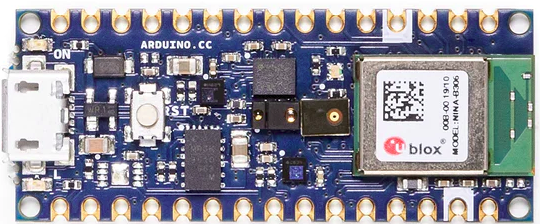
\includegraphics[scale=0.7]{./images/p.png} 
\caption{Arduino Nano 33 BLE Sense \cite{placa}.}
\label{f2}
\end{figure}
